\documentclass[12pt]{article}
\usepackage[margin=0.1in]{geometry}
\usepackage{arev}
\usepackage{pgfplots}
\usetikzlibrary{calc}
\pgfplotsset{compat=newest}

\begin{document}
\begin{figure}[h]
    \centering
    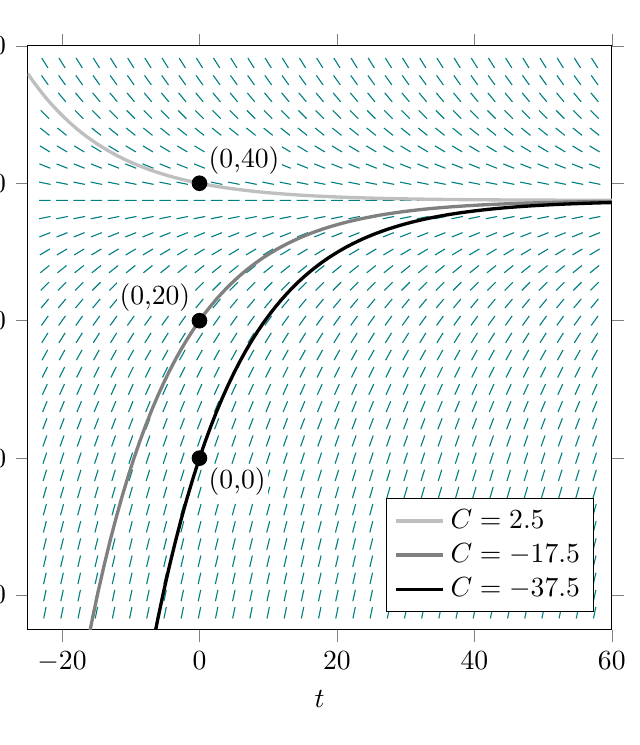
\begin{tikzpicture}[
	    trim axis left, trim axis right, % options to centre correctly
	    declare function={
		dydx(\x,\y) = 3-0.08*\y; % differential equation
		solution(\x,\c) = 37.5 + \c*exp(-0.08*x); % general solution including constant of integration
	    }
	]
        % axes settings
	\def\width{9cm} \def\height{9cm}
	\def\xmin{-25} \def\xmax{60}
	\def\ymin{-25} \def\ymax{60}
        \def\xticks{\xmin+5,\xmin+25,...,\xmax}
        \def\yticks{\ymin+5,\ymin+25,...,\ymax}

	% dummy empty axis to provide a coordinate system for the scope below
        \begin{axis}[ % axis options involving the size of the plot MUST be the same as the actual axis below
		view = {0}{90}, % set camera to point towards x-y plane
	        xmin=\xmin, xmax=\xmax, ymin=\ymin, ymax=\ymax, ticks=none, axis x line=none, axis y line=none,
	        width=\width, height=\height,
		axis equal image,
	    ]
	    \coordinate (O) at (0,0); \coordinate (X) at (1,0); \coordinate (Y) at (0,1); % basis vectors
	\end{axis}

	% must plot slope field outside of axis environment because nested \foreach is needed
	\begin{scope}[x={($(X)-(O)$)}, y={($(Y)-(O)$)}, shift={(O)}] % take the coordinate system of the dummy axis
		\def\numQuivers{32}
		\pgfmathsetmacro{\scale}{(\xmax-\xmin)/50}
		\pgfmathsetmacro{\hx}{(\xmax-\xmin)/(\numQuivers+2)} % +2 to account for the slopes at the domain edge that aren't drawn
		\pgfmathsetmacro{\hy}{(\ymax-\ymin)/(\numQuivers+2)}
		\foreach \i in {0,...,\numQuivers} {
			\foreach \j in {0,...,\numQuivers} {
			    \pgfmathsetmacro{\slope}{dydx({\hx+\xmin+\i*\hx}, {\hy+\ymin+\j*\hy})} % additional \hx and \hy offset to skip slopes at domain edge
			    % \dx and \dy are calculated from \scale * unit length tangent line
			    \pgfmathsetmacro{\dx}{\scale/sqrt((\slope)^2+1)}
			    \pgfmathsetmacro{\dy}{\scale*\slope/sqrt((\slope)^2+1)}
			    \draw[teal,shift={({\hx+\xmin+\i*\hx},{\hy+\ymin+\j*\hy})}] (-\dx/2,-\dy/2)--(\dx/2,\dy/2);
			}
		}
	\end{scope}

	% actual axis for plotting the solution, must come after slope field to provide proper masking
        \begin{axis}[
		view = {0}{90}, % set camera to point towards x-y plane
	        domain=\xmin:\xmax, xmin=\xmin, xmax=\xmax, ymin=\ymin, ymax=\ymax, xtick=\xticks, ytick=\yticks,
	        xlabel=$t$, ylabel=$w$,
	        tick align=outside,
	        width=\width, height=\height,
	        legend pos=south east, legend cell align={left},
	        axis equal image
	    ]

	    % #1: coordinates of node, #2: relative position of node label (can also be angle)
	    \newcommand\labelledPoint[2]{\node[circle, fill, inner sep=2pt, label={[fill=white,distance=1pt,inner sep=1pt]#2:{(#1)}}] at (#1){}}

            % plot initial points and corresponding solution curves
	    \addplot[very thick, black!25, samples=100] {solution(x, 2.5)};
            \labelledPoint{0,40}{above right};

	    \addplot[very thick, black!50, samples=100] {solution(x, -17.5)};
            \labelledPoint{0,20}{above left};

            \addplot[very thick, black!100, samples=100] {solution(x, -37.5)};
            \labelledPoint{0,0}{below right};

            % add legend
            \legend{$C=2.5$, $C=-17.5$, $C=-37.5$}
        \end{axis}

    \end{tikzpicture}
    \caption{Slope field of $\frac{\mathrm{d}}{t}=3-0.08w$, with general solution $w(t)=Ce^{-0.08t}+37.5$}
\end{figure}
\end{document}
